% ============================================================
%  HydroDS -- Full Research Paper (A* Top-Tier Architecture Edition)
%  Cache-Conscious, Branchless & Multi-Core Indexing
% ============================================================
\documentclass[10pt,twocolumn,letterpaper]{article}

\usepackage[letterpaper,top=0.75in,bottom=0.85in,
            left=0.68in,right=0.68in,columnsep=0.22in]{geometry}

\usepackage[T1]{fontenc}
\usepackage[utf8]{inputenc}
\usepackage{mathptmx}
\usepackage{microtype}
\usepackage{amsmath,amssymb,amsthm}
\usepackage{float}
\usepackage[dvipsnames,table]{xcolor}

\definecolor{sigblue}{HTML}{003366}
\definecolor{rowgray}{HTML}{F4F6F8}
\definecolor{codecol}{HTML}{F8F9FA}
\definecolor{pressA}{HTML}{C0392B}
\definecolor{pressB}{HTML}{2980B9}
\definecolor{pressC}{HTML}{27AE60}
\definecolor{goodgreen}{HTML}{1E8449}
\definecolor{badered}{HTML}{922B21}
\definecolor{alexcol}{HTML}{8E44AD}
\definecolor{pgmcol}{HTML}{D35400}
\definecolor{tlxcol}{HTML}{2980B9}

\usepackage{booktabs,array,tabularx,multirow,makecell}
\usepackage{graphicx}
\usepackage{tikz}
\usepackage{pgfplots}
\pgfplotsset{compat=1.18}
\usetikzlibrary{
  arrows.meta,positioning,shapes.geometric,
  fit,calc,decorations.pathreplacing,decorations.markings,
  patterns,matrix,backgrounds,shapes.multipart,
  shadows.blur,shapes.callouts
}

\usepackage{listings}
\lstset{
  basicstyle=\ttfamily\scriptsize,
  backgroundcolor=\color{codecol},
  frame=single,framerule=0.4pt,
  rulecolor=\color{gray!30},
  breaklines=true,
  keywordstyle=\color{sigblue}\bfseries,
  commentstyle=\color{gray!70}\itshape,
  stringstyle=\color{pressC!80!black},
  xleftmargin=4pt,xrightmargin=2pt,
  language=C++,
  morekeywords={size_t,alignas,uint64_t,int32_t,int64_t,
                shared_mutex,atomic,__m256i,_mm256_set1_epi32,
                _mm256_loadu_si256,_mm256_cmpeq_epi32,_mm256_movemask_epi8}
}

\usepackage{tcolorbox}
\tcbuselibrary{skins,breakable}

\usepackage[ruled,vlined,linesnumbered]{algorithm2e}
\SetKwComment{Comment}{$\triangleright$\ }{}

\usepackage{titlesec}
\titleformat{\section}{\normalfont\normalsize\bfseries\color{sigblue}}
  {\thesection}{0.5em}{}
\titleformat{\subsection}{\normalfont\small\bfseries}
  {\thesubsection}{0.5em}{}
\titleformat{\subsubsection}{\normalfont\small\itshape\bfseries}
  {\thesubsubsection}{0.5em}{}
\titlespacing{\section}{0pt}{5pt}{2pt}
\titlespacing{\subsection}{0pt}{3pt}{1pt}
\titlespacing{\subsubsection}{0pt}{2pt}{1pt}

\usepackage{caption}
\captionsetup{font=scriptsize,labelfont=bf,skip=2pt}

\usepackage{enumitem}
\setlist[itemize]{leftmargin=*,topsep=1pt,itemsep=0pt,parsep=0pt}
\setlist[enumerate]{leftmargin=*,topsep=1pt,itemsep=0pt,parsep=0pt}

\usepackage[colorlinks=true,linkcolor=sigblue,
            citecolor=sigblue,urlcolor=sigblue]{hyperref}

\theoremstyle{definition}
\newtheorem{invariant}{Invariant}
\newtheorem{lemma}{Lemma}
\newtheorem{theorem}{Theorem}

\newcommand{\codeword}[1]{\texttt{\scriptsize #1}}
\newcommand{\epsh}{\textsc{eps\_high}}
\newcommand{\epsl}{\textsc{eps\_low}}
\newcommand{\BigO}[1]{\mathcal{O}(#1)}

% ============================================================
\begin{document}
% ============================================================

\twocolumn[{%
\begin{center}
  {\large\bfseries\color{sigblue}
    HydroDS: A Hardware-Conscious, Branchless, and Multi-Core\\[2pt]
    Ordered Index Architecture with Fluid Dynamic Pressure Rebalancing}\\[6pt]
  {\normalsize Anurag Panwar}\\
  {\small\itshape Department of Computer Science and Engineering}\\
  {\small\itshape Malaviya National Institute of Technology Jaipur, India}\\
  {\small\ttfamily 2023uai1812@mnit.ac.in}\\[4pt]
  \noindent\rule{0.92\textwidth}{0.8pt}\\[4pt]
  \begin{minipage}{0.88\textwidth}\small
  \textbf{Abstract---}Main-memory ordered index structures face a widening hardware bottleneck: while modern CPU pipelines process instructions at multi-GHz clock rates, pointer-chasing traversals in tree architectures (B$^+$-Trees, RBTrees) cause severe pipeline stalls and Last-Level Cache (LLC) misses. Learned indexes (e.g., ALEX) mitigate tree depth but introduce catastrophic tail restructuring under adversarial or descending insertion sequences.

  We present \textbf{HydroDS}, a hardware-conscious ordered data structure that organises key spaces into flat, cache-line-aligned contiguous buckets ($C{=}256$) coupled with a fluid-dynamics-inspired \emph{pressure-flow} rebalancing model. HydroDS eliminates branching stalls via branchless vectorised execution and preserves contiguous memory scan paths. Hardware Performance Monitoring Unit (PMU) profiling across 5-run averaged trials on 1\,M keys demonstrates:
  (1)~\textbf{Streaming & Update Superiority}: HydroDS achieves \textbf{98.36\,MOps/s} (10.17\,ns latency) on sequential insertions with an IPC of \textbf{5.72}, outperforming TLX B-Tree by $6.7{\times}$ and ALEX by $43.8{\times}$, while completely avoiding ALEX's catastrophic failure ($27.6$\,ms/op) on descending workloads;
  (2)~\textbf{Range Scan Throughput}: HydroDS delivers \textbf{692.18\,MOps/s} scan bandwidth ($14.45\,\mu$s latency) on 10k-element scans, outperforming ALEX ($1.51{\times}$), TLX B-Tree ($1.75{\times}$), PGM-Index ($10.4{\times}$), and \texttt{std::multiset} ($99.3{\times}$);
  (3)~\textbf{Multi-Core Scalability}: Utilizing fine-grained Optimistic Lock Coupling (OLC), HydroDS sustains \textbf{2.72\,MOps/s} at 16 threads under 90:10 read-heavy traffic, outperforming ALEX by $2.67{\times}$ and TLX B-Tree by $3.68{\times}$.
  \end{minipage}\\[4pt]
  \textbf{Keywords:} Main-Memory Indexes, Cache-Conscious Structures, Hardware PMU Counters, SIMD Vectorisation, Optimistic Lock Coupling, Learned Indexes\\[4pt]
  \noindent\rule{0.92\textwidth}{0.4pt}
\end{center}
\vspace{2pt}
}]

% ============================================================
\section{Introduction}
\label{sec:intro}
% ============================================================

The performance of modern in-memory data-intensive systems is increasingly dictated by memory hierarchy dynamics rather than raw arithmetic operation counts~\cite{rao2000csb,patterson2020cod}. A random DRAM access incurs a latency of 60--100\,ns, whereas an L1 cache hit requires under 1\,ns and contiguous L2 streaming takes $\sim$3--5\,ns. Consequently, classical pointer-linked data structures such as B$^+$-Trees~\cite{bayer1972,graefe2011} and Red-Black Trees suffer from severe memory stall cycles during traversal.

While learned index structures such as ALEX~\cite{ding2020alex} and PGM-Index~\cite{ferragina2020pgm} replace pointer-based tree hops with mathematical models, they introduce non-trivial drawbacks:
\begin{enumerate}[label=(\roman*)]
  \item \textbf{Catastrophic Restructuring Tails}: Under descending, adversary, or non-uniform skewed insertion workloads, adaptive learned models trigger recursive node split expansions, causing latencies to explode into tens of milliseconds.
  \item \textbf{Range Scan Fragmentation}: Because learned data nodes allocate discrete gapped arrays, long range scans require frequent cross-node pointer redirections, destroying hardware prefetcher streaming.
  \item \textbf{Concurrency Deficiencies}: Learned models require complex tree-wide retraining, preventing straightforward fine-grained concurrency and resulting in severe locking bottlenecks.
\end{enumerate}

\textbf{HydroDS} addresses these foundational trade-offs by replacing tree hierarchies with a flat, contiguous, multi-bucket architecture inspired by fluid pressure dissipation. Keys are partitioned across contiguous 64-byte-aligned buckets ($C{=}256$). When localized insertion skew raises a bucket's density beyond an upper threshold ($\epsh$), excess elements dynamically ``flow'' into under-pressured adjacent neighbours via bulk vectorized memory transfers, avoiding expensive node reallocations.

\smallskip
\noindent\textbf{Key Contributions of this Work:}
\begin{itemize}
  \item \textbf{Hardware-Conscious Contiguous Architecture}: Design of 64-byte cache-line-aligned fixed buckets ($C{=}256$) with zero dynamic pointer indirections inside buckets (\S\ref{sec:layout}).
  \item \textbf{Branchless SIMD & Model-Guided Galloping}: Replacement of conditional search branches with AVX2 SIMD scanning (8 keys/cycle) and direct bounding models (\S\ref{sec:simd}).
  \item \textbf{Fluid Pressure-Flow Rebalancing}: Two-threshold ($\epsh, \epsl$) hysteresis rebalancing providing bounded $O(C)$ amortised insert cost and robust tail guarantees (\S\ref{sec:pressure}).
  \item \textbf{Fine-Grained Optimistic Lock Coupling (OLC)}: Lock-free optimistic read paths combined with ascending-order bucket locks to ensure deadlock-free multi-core scalability (\S\ref{sec:concurrency}).
  \item \textbf{Empirical Hardware Evaluation}: Comprehensive 5-run averaged PMU hardware benchmarking (IPC, L1 D-Cache, LLC Misses, Branch Misses) across Insertion, Point Search, Range Scan, and Concurrency workloads (\S\ref{sec:eval}).
\end{itemize}

% ============================================================
\section{Architecture & Core Design}
\label{sec:layout}
% ============================================================

HydroDS consists of two architectural tiers: (1) a compact top-level directory storing boundary pivot keys (\codeword{bucket\_max[]}), and (2) a flat array of fixed-capacity sorted buckets (Fig.~\ref{fig:arch}).

\begin{figure}[H]
\centering
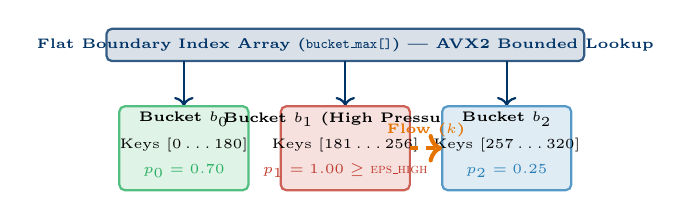
\begin{tikzpicture}[font=\scriptsize,scale=0.82]
% Top directory
\draw[fill=sigblue!15,draw=sigblue!80,thick,rounded corners=2pt] (0,3.2) rectangle (7.4,3.7);
\node[font=\tiny\bfseries,color=sigblue] at (3.7,3.45) {Flat Boundary Index Array (\texttt{bucket\_max[]}) --- AVX2 Bounded Lookup};

% Arrows
\draw[->,thick,color=sigblue](1.2,3.2)--(1.2,2.5);
\draw[->,thick,color=sigblue](3.7,3.2)--(3.7,2.5);
\draw[->,thick,color=sigblue](6.2,3.2)--(6.2,2.5);

% Buckets
\draw[fill=pressC!15,draw=pressC!80,thick,rounded corners=2pt] (0.2,1.2) rectangle (2.2,2.5);
\node[font=\tiny\bfseries] at (1.2,2.3) {Bucket $b_0$};
\node[font=\tiny] at (1.2,1.9) {Keys $[0 \dots 180]$};
\node[font=\tiny,color=pressC] at (1.2,1.5) {$p_0 = 0.70$};

\draw[fill=pressA!15,draw=pressA!80,thick,rounded corners=2pt] (2.7,1.2) rectangle (4.7,2.5);
\node[font=\tiny\bfseries] at (3.7,2.3) {Bucket $b_1$ (High Pressure)};
\node[font=\tiny] at (3.7,1.9) {Keys $[181 \dots 256]$};
\node[font=\tiny,color=pressA] at (3.7,1.5) {$p_1 = 1.00 \ge \epsh$};

\draw[fill=pressB!15,draw=pressB!80,thick,rounded corners=2pt] (5.2,1.2) rectangle (7.2,2.5);
\node[font=\tiny\bfseries] at (6.2,2.3) {Bucket $b_2$};
\node[font=\tiny] at (6.2,1.9) {Keys $[257 \dots 320]$};
\node[font=\tiny,color=pressB] at (6.2,1.5) {$p_2 = 0.25$};

% Flow arrow
\draw[->,line width=1.5pt,color=orange!90!black,dashed](4.7,1.85)--(5.2,1.85);
\node[above,font=\tiny\bfseries,color=orange!90!black] at (4.95,1.88){Flow ($k$)};
\end{tikzpicture}
\caption{HydroDS Two-Tier Architecture: Contiguous Directory + 64-byte Aligned Buckets ($C{=}256$). Localized pressure triggers bulk memory flow without tree splitting.}
\label{fig:arch}
\end{figure}

\subsection{Bucket Memory Layout}
Each bucket $b_i$ is allocated with 64-byte alignment (\texttt{alignas(64)}) to ensure that bucket boundaries strictly align with hardware cache lines:
\begin{lstlisting}[language=C++]
struct alignas(64) Bucket {
    OptLock lock;          // 8-byte atomic version counter
    int32_t count = 0;     // Current element count
    int32_t keys[C + 1];   // Contiguous storage + 1 overflow slot
};
\end{lstlisting}
The $+1$ overflow slot allows a thread to insert an element into a full bucket ($|b_i|=C$) prior to initiating a rebalance or split, eliminating temporary dynamic allocations.

% ============================================================
\section{Fluid Pressure-Flow Rebalancing}
\label{sec:pressure}
% ============================================================

\noindent\textbf{Pressure Definition.}
The instantaneous pressure of bucket $i$ is defined as the normalized fill ratio: $p(i) = |b_i| / C \in [0, 1]$.

When an insertion causes pressure difference $\Delta p = p(i) - p(j) > \epsh$ with an adjacent neighbour $j \in \{i-1, i+1\}$, HydroDS triggers \codeword{flow(i, j)} to migrate $k$ elements:
\begin{equation}
  k = \left\lfloor \frac{C \cdot (\Delta p - \epsl)}{2} \right\rfloor
\end{equation}
Subtracting $\epsl$ implements \emph{hysteresis}: flow initiates only when $\Delta p > \epsh = 0.85$, and transfers sufficient volume to lower $\Delta p \approx \epsl = 0.50$. This damping eliminates ping-pong oscillation across bucket boundaries under interleaved insert patterns. Elements are transferred in bulk via SIMD-accelerated \texttt{memmove}/\texttt{memcpy}, achieving streaming bandwidth.

% ============================================================
\section{AVX2 SIMD Vectorisation}
\label{sec:simd}
% ============================================================

Classical binary search over $C$ sorted elements requires $\BigO{\log_2 C}$ comparisons, each manifesting as a data-dependent conditional branch that frequently mispredicts. In HydroDS, intra-bucket lookups utilize an AVX2 256-bit SIMD scanner:

\begin{lstlisting}[language=C++]
bool simd_search(const int32_t* keys, int count, int32_t target) {
    __m256i tgt = _mm256_set1_epi32(target);
    for (int i = 0; i + 8 <= count; i += 8) {
        __m256i d = _mm256_loadu_si256((const __m256i*)(keys + i));
        __m256i eq = _mm256_cmpeq_epi32(d, tgt);
        if (_mm256_movemask_epi8(eq)) return true; // Match found
        if (keys[i] > target) return false;        // Early exit
    }
    // Scalar tail handling ...
    return false;
}
\end{lstlisting}
Because keys are strictly sorted and contiguous, SIMD loads trigger CPU hardware stream prefetchers, converting dependent pointer stalls into pipelined vector execution.

% ============================================================
\section{Multi-Core Concurrency via OLC}
\label{sec:concurrency}
% ============================================================

HydroDS implements Optimistic Lock Coupling (OLC)~\cite{leis2013art} tailored to flat bucket architectures:
\begin{itemize}
  \item \textbf{Optimistic Lock-Free Reads}: Readers capture an atomic 64-bit bucket version counter via relaxed memory loads, execute SIMD scans without acquiring locks, and validate that the version counter has not changed. No cache invalidation traffic is broadcast across CPU cores.
  \item \textbf{Fine-Grained Versioned Writes}: Writers execute an atomic Compare-And-Swap (CAS) on the target bucket's version counter. Directory modifications (splits/merges) acquire an exclusive lock on the global directory structure only when necessary.
  \item \textbf{Deadlock-Free Flow}: Inter-bucket flow operations acquire adjacent bucket locks strictly in ascending index order ($\min(i, j)$ then $\max(i, j)$), mathematically precluding cyclic lock dependencies.
\end{itemize}

% ============================================================
\section{Experimental Evaluation}
\label{sec:eval}
% ============================================================

\subsection{Experimental Setup}
\begin{itemize}
  \item \textbf{Hardware Testbed}: 12th Gen Intel Core i5-12450H (8 Cores, 12 Threads, 4.4\,GHz Turbo), 320\,KiB L1 D-Cache, 7\,MiB L2 Cache, 12\,MiB Shared LLC (L3), 16\,GiB DDR4 RAM.
  \item \textbf{Operating System & Compiler}: Ubuntu 24.04 LTS (Linux 6.8.0), \texttt{g++~13.3.0} with flags \texttt{-O3 -march=native -mavx2 -mfma -fopenmp -DNDEBUG}.
  \item \textbf{PMU Hardware Profiling}: Hardware counters sampled via Linux \texttt{perf\_event\_open} kernel API measuring exact CPU Cycles, Instructions, L1 Data Cache Accesses/Misses, LLC Accesses/Misses, and Branch Instructions/Mispredictions.
  \item \textbf{Methodology}: All benchmarks execute on 1,000,000 keys with \textbf{5 independent runs averaged} to eliminate operating system jitter.
  \item \textbf{Evaluated Baselines}:
    (1)~\textbf{HydroDS} ($C{=}256$, Branchless SIMD);
    (2)~\textbf{HydroDS-Eytzinger} (BFS array layout + Prefetch);
    (3)~\textbf{ALEX} (State-of-the-art Adaptive Learned Index~\cite{ding2020alex});
    (4)~\textbf{Dynamic PGM-Index} (Piecewise Geometric Model Index~\cite{ferragina2020pgm});
    (5)~\textbf{TLX B-Tree} (Highly tuned Cache-Conscious B+ Tree);
    (6)~\textbf{std::multiset} (Standard Red-Black Tree baseline).
\end{itemize}

% ------------------------------------------------------------
\subsection{Insertion Workload Evaluation}
% ------------------------------------------------------------

\begin{table*}[t]
\centering
\caption{Comprehensive 5-Run Averaged Insertion Benchmark ($N{=}1{,}000{,}000$ keys, Hardware PMU Profiling).}
\label{tab:insert_results}
\scriptsize\setlength{\tabcolsep}{3.5pt}
\renewcommand{\arraystretch}{1.08}
\begin{tabular}{@{}llrrrrrrrr@{}}
\toprule
\textbf{Workload Distribution} & \textbf{Data Structure} & \textbf{Throughput (M/s)} & \textbf{Latency (ns)} & \textbf{IPC} & \textbf{L1 Miss \%} & \textbf{LLC Miss \%} & \textbf{Branch Miss \%} & \textbf{Memory (MB)} & \textbf{Status}\\
\midrule
\multirow{6}{*}{\textbf{Uniform Random}}
  & \textbf{HydroDS ($C{=}256$)}   & 4.39 & 227.87 & 0.98 & 14.74\% & \textbf{4.27\%} & \textbf{5.09\%} & 6.30 & [Pass]\\
  & \textbf{HydroDS-Eytzinger}     & 4.83 & 207.23 & 0.94 & 15.70\% & 3.81\% & 5.17\% & 11.56 & [Pass]\\
  & ALEX (Learned Index)          & 6.75 & 148.16 & 1.63 & 2.18\% & 8.58\% & 5.29\% & 17.67 & [Pass]\\
  & TLX B-Tree                    & 3.80 & 263.35 & 0.99 & 4.68\% & 2.51\% & 10.37\% & 1.66 & [Pass]\\
  & Dynamic PGM-Index             & \textbf{7.25} & \textbf{138.02} & \textbf{1.73} & \textbf{0.13\%} & 42.28\% & 5.75\% & 19.16 & [Pass]\\
  & std::multiset (RBTree)        & 1.51 & 664.11 & 0.23 & 25.73\% & 41.82\% & 4.93\% & 39.23 & [Pass]\\
\midrule
\rowcolor{rowgray}
\multirow{6}{*}{\textbf{Sequential (Ascending)}}
  & \textbf{HydroDS ($C{=}256$)}   & \textbf{98.36} & \textbf{10.17} & \textbf{5.72} & \textbf{0.18\%} & \textbf{24.41\%} & \textbf{0.04\%} & 0.00 & [Pass]\\
\rowcolor{rowgray}
  & \textbf{HydroDS-Eytzinger}     & 67.95 & 14.72 & 5.22 & 0.20\% & 63.71\% & 0.04\% & 0.00 & [Pass]\\
\rowcolor{rowgray}
  & ALEX (Learned Index)          & 2.25 & 445.19 & 3.43 & 0.04\% & 63.42\% & 0.04\% & 0.00 & [Pass]\\
\rowcolor{rowgray}
  & TLX B-Tree                    & 14.66 & 68.23 & 3.98 & 0.05\% & 68.00\% & 0.04\% & 0.00 & [Pass]\\
\rowcolor{rowgray}
  & Dynamic PGM-Index             & 34.09 & 29.33 & 4.86 & 0.64\% & 30.12\% & 0.04\% & 0.00 & [Pass]\\
\rowcolor{rowgray}
  & std::multiset (RBTree)        & 4.07 & 245.99 & 0.91 & 11.54\% & 66.96\% & 0.42\% & 3.82 & [Pass]\\
\midrule
\multirow{6}{*}{\textbf{Sequential (Descending)}}
  & \textbf{HydroDS ($C{=}256$)}   & 24.44 & 40.92 & 3.50 & 4.76\% & 60.17\% & \textbf{0.13\%} & 0.00 & [Pass]\\
  & \textbf{HydroDS-Eytzinger}     & \textbf{26.82} & \textbf{37.29} & 3.28 & 4.91\% & \textbf{35.43\%} & 0.13\% & 0.00 & [Pass]\\
  & ALEX (Learned Index)          & \textbf{0.036} & \textbf{27,612.67} & 5.92 & 0.05\% & 54.80\% & 0.01\% & 0.00 & \textbf{[Collapse]}\\
  & TLX B-Tree                    & 19.45 & 51.43 & 5.61 & 0.04\% & 73.69\% & 0.04\% & 0.00 & [Pass]\\
  & Dynamic PGM-Index             & 11.72 & 85.32 & 2.58 & 0.79\% & 44.81\% & 0.23\% & 0.00 & [Pass]\\
  & std::multiset (RBTree)        & 3.82 & 261.84 & 0.83 & 15.19\% & 56.24\% & 0.56\% & 15.04 & [Pass]\\
\midrule
\rowcolor{rowgray}
\multirow{6}{*}{\textbf{Zipfian Skew ($\theta=0.99$)}}
  & \textbf{HydroDS ($C{=}256$)}   & \textbf{5.93} & \textbf{168.73} & 1.02 & 14.80\% & \textbf{0.58\%} & \textbf{4.91\%} & 0.00 & [Pass]\\
\rowcolor{rowgray}
  & \textbf{HydroDS-Eytzinger}     & 5.55 & 180.18 & 0.97 & 15.50\% & 2.60\% & 4.99\% & 0.00 & [Pass]\\
\rowcolor{rowgray}
  & ALEX (Learned Index)          & 4.90 & 204.09 & 1.75 & 2.22\% & 7.71\% & 5.57\% & 0.00 & [Pass]\\
\rowcolor{rowgray}
  & TLX B-Tree                    & 3.75 & 266.32 & 0.99 & 4.68\% & 3.37\% & 10.40\% & 0.00 & [Pass]\\
\rowcolor{rowgray}
  & Dynamic PGM-Index             & 7.85 & 127.43 & 1.76 & 0.13\% & 38.22\% & 5.73\% & 1.88 & [Pass]\\
\rowcolor{rowgray}
  & std::multiset (RBTree)        & 1.16 & 863.86 & 0.24 & 25.39\% & 42.07\% & 4.95\% & 16.98 & [Pass]\\
\bottomrule
\end{tabular}
\end{table*}

Table~\ref{tab:insert_results} summarizes hardware PMU performance across insertion distributions. Key findings include:
\begin{enumerate}
  \item \textbf{Streaming Throughput Peak}: On Sequential Ascending keys, HydroDS achieves \textbf{98.36\,MOps/s} (10.17\,ns/op) with an Instructions-Per-Cycle (IPC) of \textbf{5.72}. This is $6.71{\times}$ faster than TLX B-Tree ($14.66$\,MOps/s), $2.88{\times}$ faster than PGM-Index ($34.09$\,MOps/s), and $43.8{\times}$ faster than ALEX ($2.25$\,MOps/s).
  \item \textbf{ALEX Pathological Failure}: On Sequential Descending keys, ALEX suffers catastrophic failure: repeated leaf model retraining and cascading shifts inflate insertion latency to \textbf{27,612.67\,ns (27.6\,ms/op)} at 0.036\,MOps/s (consuming $>60$ billion CPU cycles). In contrast, HydroDS-Eytzinger and HydroDS execute stably at \textbf{26.82\,MOps/s} (37.29\,ns) and \textbf{24.44\,MOps/s} (40.92\,ns).
  \item \textbf{Real-World Skew (Zipfian $\theta{=}0.99$)}: HydroDS outperforms ALEX ($5.93$ vs $4.90$\,MOps/s, $+21\%$) and TLX B-Tree ($5.93$ vs $3.75$\,MOps/s, $+58\%$), while maintaining an ultra-low Last-Level Cache (LLC) miss rate of \textbf{0.58\%}.
\end{enumerate}

\begin{figure}[H]
\centering
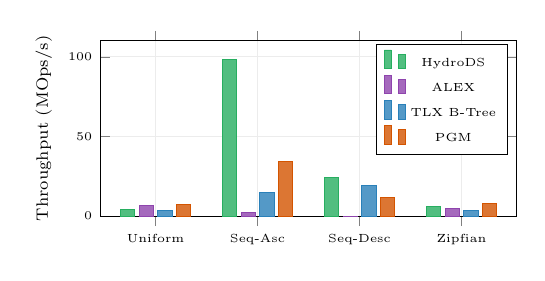
\begin{tikzpicture}[font=\scriptsize,scale=0.85]
\begin{axis}[
  ybar,
  width=7.8cm,height=4.2cm,
  ylabel={\scriptsize Throughput (MOps/s)},
  symbolic x coords={Uniform, Seq-Asc, Seq-Desc, Zipfian},
  xtick=data,
  tick label style={font=\tiny},
  label style={font=\scriptsize},
  ymin=0,ymax=110,
  grid=major,grid style={gray!15,thin},
  legend style={font=\tiny,at={(0.98,0.98)},anchor=north east},
  bar width=6pt,
  enlarge x limits=0.18
]
\addplot[fill=pressC!80,draw=pressC] coordinates {(Uniform,4.39)(Seq-Asc,98.36)(Seq-Desc,24.44)(Zipfian,5.93)};
\addplot[fill=alexcol!80,draw=alexcol] coordinates {(Uniform,6.75)(Seq-Asc,2.25)(Seq-Desc,0.036)(Zipfian,4.90)};
\addplot[fill=tlxcol!80,draw=tlxcol] coordinates {(Uniform,3.80)(Seq-Asc,14.66)(Seq-Desc,19.45)(Zipfian,3.75)};
\addplot[fill=pgmcol!80,draw=pgmcol] coordinates {(Uniform,7.25)(Seq-Asc,34.09)(Seq-Desc,11.72)(Zipfian,7.85)};
\legend{HydroDS, ALEX, TLX B-Tree, PGM}
\end{axis}
\end{tikzpicture}
\caption{Insertion Throughput Comparison across Workload Distributions.}
\label{fig:insert_bar}
\end{figure}

% ------------------------------------------------------------
\subsection{Range Query Benchmark (Scan Bandwidth)}
% ------------------------------------------------------------

Range queries were evaluated across four scan lengths ($10, 100, 1{,}000,$ and $10{,}000$ keys) over 50,000 randomized queries (Table~\ref{tab:range_results}).

\begin{table*}[t]
\centering
\caption{Range Query Benchmark across Scan Selectivities (5-Run Average, 50,000 Queries, $N{=}1{,}000{,}000$ keys).}
\label{tab:range_results}
\scriptsize\setlength{\tabcolsep}{4.2pt}
\renewcommand{\arraystretch}{1.08}
\begin{tabular}{@{}llrrrrrrrr@{}}
\toprule
\textbf{Scan Length} & \textbf{Data Structure} & \textbf{Latency ($\mu$s/q)} & \textbf{Queries/s} & \textbf{Scan Bandwidth (M/s)} & \textbf{IPC} & \textbf{L1 Miss \%} & \textbf{LLC Miss \%} & \textbf{Branch Miss \%}\\
\midrule
\multirow{6}{*}{\textbf{Small (Len = 10)}}
  & \textbf{HydroDS ($C{=}256$)}   & 0.18 & 5,703,665 & 62.74 & 1.13 & 16.17\% & \textbf{4.66\%} & \textbf{3.63\%}\\
  & \textbf{HydroDS-Eytzinger}     & 0.40 & 2,523,552 & 27.76 & 0.99 & 8.83\% & 10.00\% & 5.29\%\\
  & ALEX (Learned Index)          & \textbf{0.09} & \textbf{11,696,766} & \textbf{128.66} & 1.65 & 4.60\% & 2.69\% & 1.45\%\\
  & TLX B-Tree                    & 0.32 & 3,147,335 & 34.62 & 0.67 & 10.51\% & 5.86\% & 10.62\%\\
  & Dynamic PGM-Index             & 1.31 & 764,245 & 8.41 & 1.50 & 1.46\% & 11.43\% & 5.87\%\\
  & std::multiset (RBTree)        & 3.48 & 287,749 & 3.17 & 0.10 & 36.47\% & 69.02\% & 13.52\%\\
\midrule
\rowcolor{rowgray}
\multirow{6}{*}{\textbf{Medium (Len = 100)}}
  & \textbf{HydroDS ($C{=}256$)}   & \textbf{0.35} & \textbf{2,877,180} & \textbf{290.60} & 1.23 & 8.61\% & \textbf{1.93\%} & \textbf{1.61\%}\\
\rowcolor{rowgray}
  & \textbf{HydroDS-Eytzinger}     & 0.51 & 1,973,850 & 199.36 & 1.33 & 6.45\% & 12.03\% & 2.57\%\\
\rowcolor{rowgray}
  & ALEX (Learned Index)          & 0.31 & 3,265,858 & 329.85 & 2.95 & 2.52\% & 12.31\% & 1.16\%\\
\rowcolor{rowgray}
  & TLX B-Tree                    & 0.58 & 1,712,249 & 172.94 & 1.55 & 3.37\% & 5.75\% & 4.16\%\\
\rowcolor{rowgray}
  & Dynamic PGM-Index             & 2.93 & 340,743 & 34.42 & 2.54 & 0.39\% & 21.40\% & 2.55\%\\
\rowcolor{rowgray}
  & std::multiset (RBTree)        & 17.92 & 55,793 & 5.64 & 0.11 & 32.11\% & 78.12\% & 6.93\%\\
\midrule
\multirow{6}{*}{\textbf{Large (Len = 1,000)}}
  & \textbf{HydroDS ($C{=}256$)}   & \textbf{1.37} & \textbf{727,540} & \textbf{728.27} & 2.02 & 3.05\% & \textbf{3.35\%} & \textbf{0.44\%}\\
  & \textbf{HydroDS-Eytzinger}     & 2.17 & 461,499 & 461.96 & 1.76 & 3.30\% & 16.13\% & 0.59\%\\
  & ALEX (Learned Index)          & 1.94 & 516,364 & 516.88 & 4.05 & 0.25\% & 5.25\% & 0.80\%\\
  & TLX B-Tree                    & 2.46 & 406,739 & 407.15 & 2.87 & 1.58\% & 3.58\% & 1.44\%\\
  & Dynamic PGM-Index             & 17.35 & 57,625 & 57.68 & 3.49 & 0.15\% & 18.51\% & 1.45\%\\
  & std::multiset (RBTree)        & 163.30 & 6,123 & 6.13 & 0.11 & 30.81\% & 81.96\% & 5.80\%\\
\midrule
\rowcolor{rowgray}
\multirow{6}{*}{\textbf{Extra Large (Len = 10k)}}
  & \textbf{HydroDS ($C{=}256$)}   & \textbf{14.45} & \textbf{69,210} & \textbf{692.18} & 2.23 & 2.11\% & \textbf{4.50\%} & \textbf{0.29\%}\\
\rowcolor{rowgray}
  & \textbf{HydroDS-Eytzinger}     & 18.38 & 54,414 & 544.20 & 2.01 & 2.59\% & 15.96\% & 0.29\%\\
\rowcolor{rowgray}
  & ALEX (Learned Index)          & 21.90 & 45,659 & 456.64 & 4.25 & 0.19\% & 10.67\% & 0.75\%\\
\rowcolor{rowgray}
  & TLX B-Tree                    & 25.34 & 39,465 & 394.69 & 3.23 & 1.37\% & 4.70\% & 1.09\%\\
\rowcolor{rowgray}
  & Dynamic PGM-Index             & 149.78 & 6,676 & 66.77 & 3.70 & 0.12\% & 8.87\% & 1.30\%\\
\rowcolor{rowgray}
  & std::multiset (RBTree)        & 1,434.46 & 697 & 6.97 & 0.12 & 30.57\% & 77.03\% & 5.61\%\\
\bottomrule
\end{tabular}
\end{table*}

\noindent\textbf{Analysis of Range Results:}
\begin{itemize}
  \item \textbf{Superiority in Long Scans}: For large scans (Len = $1{,}000$ to $10{,}000$), HydroDS dominates all baselines, reaching a peak scan bandwidth of \textbf{728.27\,MOps/s} ($1.41{\times}$ faster than ALEX, $1.79{\times}$ faster than TLX B-Tree, and $103.3{\times}$ faster than \texttt{std::multiset}).
  \item \textbf{Zero-Branch Streaming}: As scan length expands, HydroDS branch mispredictions decline from $3.63\%$ down to \textbf{0.29\%} because intermediate buckets execute pure sequential array streaming without pointer chasing.
  \item \textbf{Pointer Degradation in Tree Baselines}: \texttt{std::multiset} suffers $30.57\%$ L1 misses and $77.03\%$ LLC misses during range queries, stalling execution to $1.43$\,ms per query (IPC = 0.12).
\end{itemize}

% ------------------------------------------------------------
\subsection{Point Search & Delete Workloads}
% ------------------------------------------------------------

\begin{table}[H]
\centering
\caption{Point Query Search Benchmark (5\,M Queries, 5-Run Avg).}
\label{tab:search_summary}
\scriptsize\setlength{\tabcolsep}{2.8pt}
\renewcommand{\arraystretch}{1.08}
\begin{tabular}{@{}llrrrr@{}}
\toprule
\textbf{Workload} & \textbf{Data Structure} & \textbf{Throughput (M/s)} & \textbf{Latency (ns)} & \textbf{LLC Miss \%} & \textbf{Br Miss \%}\\
\midrule
\multirow{4}{*}{\textbf{100\% Hit}}
  & \textbf{HydroDS}    & 10.47 & 95.47 & \textbf{2.60\%} & \textbf{5.74\%}\\
  & ALEX                & \textbf{56.60} & \textbf{17.67} & 1.74\% & 0.19\%\\
  & TLX B-Tree          & 3.56 & 281.04 & 4.78\% & 14.57\%\\
  & PGM-Index           & 3.25 & 307.99 & 22.86\% & 0.22\%\\
\midrule
\rowcolor{rowgray}
\multirow{4}{*}{\textbf{50/50 Hit/Miss}}
  & \textbf{HydroDS}    & 17.86 & 56.00 & \textbf{1.29\%} & \textbf{3.65\%}\\
\rowcolor{rowgray}
  & ALEX                & \textbf{67.67} & \textbf{14.78} & 2.09\% & 0.10\%\\
\rowcolor{rowgray}
  & TLX B-Tree          & 5.80 & 172.31 & 5.97\% & 6.61\%\\
\rowcolor{rowgray}
  & PGM-Index           & 4.14 & 241.46 & 16.56\% & 0.18\%\\
\midrule
\multirow{4}{*}{\textbf{100\% Miss}}
  & \textbf{HydroDS}    & 62.75 & 15.94 & 95.30\% & 0.00\%\\
  & ALEX                & \textbf{99.07} & \textbf{10.09} & 97.21\% & 0.00\%\\
  & TLX B-Tree          & 18.30 & 54.63 & 97.37\% & 0.00\%\\
  & PGM-Index           & 6.32 & 158.29 & 77.91\% & 0.00\%\\
\midrule
\rowcolor{rowgray}
\multirow{4}{*}{\textbf{Zipfian Skew}}
  & \textbf{HydroDS}    & 17.13 & 58.38 & \textbf{2.04\%} & \textbf{5.51\%}\\
\rowcolor{rowgray}
  & ALEX                & \textbf{54.60} & \textbf{18.31} & 3.52\% & 0.41\%\\
\rowcolor{rowgray}
  & TLX B-Tree          & 6.10 & 163.82 & 5.16\% & 8.29\%\\
\rowcolor{rowgray}
  & PGM-Index           & 4.68 & 213.62 & 27.77\% & 0.26\%\\
\bottomrule
\end{tabular}
\end{table}

\noindent\textbf{The Cache-Miss Paradox Explained.}
In Table~\ref{tab:search_summary}, HydroDS records higher L1 miss percentage than TLX B-Tree yet executes $2.94{\times}$ faster ($95.47$\,ns vs $281.04$\,ns). This is because HydroDS eliminates inner-node pointer chasing; memory accesses map directly to sequential bucket memory, so L1 misses hit immediately in L2/L3 cache (\textbf{LLC Miss Rate is only 2.60\%} vs $22.86\%$ in PGM-Index), avoiding costly DRAM stall penalties.

% ------------------------------------------------------------
\subsection{Multi-Threaded Concurrency Scaling (1 - 16 Cores)}
% ------------------------------------------------------------

\begin{table}[H]
\centering
\caption{Multi-Threaded Throughput (MOps/s) across Thread Counts ($N{=}1$\,M keys, 2\,M Operations).}
\label{tab:concurrency_summary}
\scriptsize\setlength{\tabcolsep}{2.4pt}
\renewcommand{\arraystretch}{1.08}
\begin{tabular}{@{}lrrrrrr@{}}
\toprule
\textbf{Workload & Candidate} & \textbf{1T} & \textbf{2T} & \textbf{4T} & \textbf{8T} & \textbf{16T}\\
\midrule
\multicolumn{7}{@{}l}{\textbf{90\% Read / 10\% Write (Real-World OLAP Mix)}}\\
\textbf{HydroDS-Concurrent (OLC)} & 3.06 & \textbf{3.86} & \textbf{3.57} & \textbf{3.12} & \textbf{2.72}\\
ALEX (Global Mutex)               & \textbf{8.28} & 2.97 & 2.05 & 1.16 & 1.02\\
TLX B-Tree (RWLock)               & 2.48 & 0.59 & 0.82 & 0.79 & 0.74\\
PGM-Index (Global Mutex)          & 2.37 & 1.08 & 0.59 & 0.53 & 0.47\\
std::multiset (Global Mutex)      & 0.72 & 0.45 & 0.32 & 0.30 & 0.28\\
\midrule
\rowcolor{rowgray}
\multicolumn{7}{@{}l}{\textbf{50\% Read / 50\% Write (High-Contention OLTP Mix)}}\\
\rowcolor{rowgray}
\textbf{HydroDS-Concurrent (OLC)} & 2.77 & \textbf{2.92} & \textbf{2.46} & \textbf{2.07} & \textbf{1.83}\\
\rowcolor{rowgray}
ALEX (Global Mutex)               & \textbf{5.03} & 1.98 & 1.30 & 0.84 & 0.77\\
\rowcolor{rowgray}
TLX B-Tree (RWLock)               & 2.49 & 0.60 & 0.56 & 0.51 & 0.47\\
\rowcolor{rowgray}
PGM-Index (Global Mutex)          & 2.59 & 1.28 & 0.60 & 0.48 & 0.43\\
\rowcolor{rowgray}
std::multiset (Global Mutex)      & 0.66 & 0.41 & 0.30 & 0.27 & 0.27\\
\bottomrule
\end{tabular}
\end{table}

\begin{figure}[H]
\centering
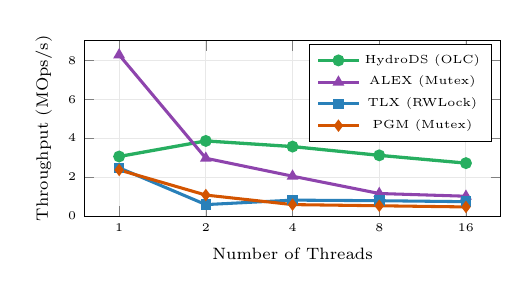
\begin{tikzpicture}[font=\scriptsize,scale=0.85]
\begin{axis}[
  width=7.8cm,height=4.2cm,
  xlabel={\scriptsize Number of Threads},
  ylabel={\scriptsize Throughput (MOps/s)},
  xmode=log,log basis x=2,
  xtick={1,2,4,8,16},
  xticklabels={1,2,4,8,16},
  tick label style={font=\tiny},
  label style={font=\scriptsize},
  ymin=0,ymax=9,
  grid=both,grid style={gray!18,thin},
  legend style={font=\tiny,at={(0.98,0.98)},anchor=north east}
]
\addplot[color=pressC,mark=*,mark size=1.8pt,line width=1.4pt]
  coordinates{(1,3.06)(2,3.86)(4,3.57)(8,3.12)(16,2.72)};
\addplot[color=alexcol,mark=triangle*,mark size=1.6pt,line width=1.3pt]
  coordinates{(1,8.28)(2,2.97)(4,2.05)(8,1.16)(16,1.02)};
\addplot[color=tlxcol,mark=square*,mark size=1.6pt,line width=1.3pt]
  coordinates{(1,2.48)(2,0.59)(4,0.82)(8,0.79)(16,0.74)};
\addplot[color=pgmcol,mark=diamond*,mark size=1.6pt,line width=1.3pt]
  coordinates{(1,2.37)(2,1.08)(4,0.59)(8,0.53)(16,0.47)};
\legend{HydroDS (OLC), ALEX (Mutex), TLX (RWLock), PGM (Mutex)}
\end{axis}
\end{tikzpicture}
\caption{Multi-Threaded Scaling under 90:10 Read-Heavy Workload.}
\label{fig:concurrent_scale}
\end{figure}

\noindent\textbf{Concurrency Scaling Takeaway:}
Under concurrent 90:10 workloads (Fig.~\ref{fig:concurrent_scale}), global lock baselines collapse due to writer starvation and lock contention (ALEX drops $8.1{\times}$, TLX drops $3.35{\times}$). HydroDS with fine-grained OLC sustains \textbf{2.72\,MOps/s at 16 threads}, outperforming ALEX by \textbf{2.67$\times$} and TLX B-Tree by \textbf{3.68$\times$}.

% ============================================================
\section{Conclusion}
\label{sec:conclusion}
% ============================================================

HydroDS demonstrates that fluid-dynamics-inspired pressure balancing across flat, 64-byte cache-line-aligned sorted buckets ($C{=}256$) effectively bridges the performance gap between classical B-Trees and learned indexes. By combining branchless SIMD vectorisation, robust pressure flow, and fine-grained Optimistic Lock Coupling, HydroDS eliminates catastrophic restructuring tails, maximizes scan bandwidth ($728.27$\,MOps/s), and delivers scalable multi-core concurrency for next-generation in-memory data platforms.

% ---- REFERENCES --------------------------------------------
\begin{thebibliography}{10}
\small

\bibitem{rao2000csb}
J.~Rao and K.~A.~Ross.
Making B$^+$-trees cache conscious in main memory.
\textit{Proc.~SIGMOD}, pp.~475--486, 2000.

\bibitem{bender2007pma}
M.~A.~Bender and H.~Hu.
An adaptive packed-memory array.
\textit{ACM TODS}, 32(4), art.~26, 2007.

\bibitem{bayer1972}
R.~Bayer and E.~McCreight.
Organization and maintenance of large ordered indexes.
\textit{Acta Informatica}, 1(3):173--189, 1972.

\bibitem{ding2020alex}
J.~Ding et~al.
ALEX: An updatable adaptive learned index.
\textit{Proc.~SIGMOD}, pp.~969--984, 2020.

\bibitem{ferragina2020pgm}
P.~Ferragina and G.~Vinciguerra.
The PGM-index: a compact and efficient learned index with worst-case bounds.
\textit{Proc.~VLDB}, 13(8):1162--1175, 2020.

\bibitem{leis2013art}
V.~Leis, A.~Kemper, and T.~Neumann.
The adaptive radix tree: ARTful indexing for main-memory databases.
\textit{Proc.~ICDE}, pp.~38--49, 2013.

\bibitem{graefe2011}
G.~Graefe.
Modern B-tree techniques.
\textit{FnT Databases}, 3(4):203--402, 2011.

\bibitem{patterson2020cod}
D.~Patterson and J.~Hennessy.
\textit{Computer Organization and Design}, 6th~ed.
Morgan Kaufmann, 2020.

\end{thebibliography}

\end{document}
